\documentclass{article}
\usepackage{amsmath, amssymb, ctex, graphicx, color}
\usepackage[margin=1in]{geometry}
\usepackage{setspace} % 行距控制
\usepackage{array}
\usepackage{makecell}

\usepackage{algorithm}
\usepackage{algpseudocode}
\usepackage{xcolor}
% 把默认注释符号 ▷ 改成行尾 // 等宽紫色，并右对齐
\renewcommand{\algorithmiccomment}[1]{\hfill\texttt{\textcolor{violet}{// #1}}}
% 定义 Input / Output 关键字（默认是 Require / Ensure）
\algnewcommand\algorithmicinput{\textbf{Input:}}
\algnewcommand\algorithmicoutput{\textbf{Output:}}
\algnewcommand\Input{\item[\algorithmicinput]}
\algnewcommand\Output{\item[\algorithmicoutput]}

\usepackage{titling}\setlength{\droptitle}{-2cm} 
\title{Ch7. Gradient Descent \\ 
Section 7.3. Convergence \\
第7章-梯度下降 -- 第7.3节-收敛性}
\author{《深度学习基础》课程小组}
% \date{}
 
\begin{document}
\maketitle
% \tableofcontents

\setlength{\parindent}{0pt} % 取消首行缩进
\setlength{\parskip}{1.5em} % 设置段落之间的距离

\noindent\rule{\linewidth}{0.4pt}

\section{P1}

When applying gradient descent in practice, we need to choose a value for the learning rate parameter $\eta$. Consider the simple error surface depicted in \textbf{Figure 7.3} for a hypothetical two-dimensional weight space in which the curvature of $E$ varies significantly with direction, creating a `valley'. At most points on the error surface, the local gradient vector for batch gradient descent, which is perpendicular to the local contour, does not point directly towards the minimum. Intuitively we might expect that increasing the value of $\eta$ should lead to bigger steps through weight space and hence faster convergence. However, the successive steps oscillate back and forth across the valley, and if we increase $\eta$ too much, those oscillations will become divergent. Because $\eta$ must be kept sufficiently small to avoid divergent oscillations across the valley, progress along the valley is very slow. Gradient descent then takes many small steps to reach the minimum and is a very inefficient procedure.

Figure 7.3 Caption: Schematic illustration of fixed-step gradient descent for an error function that has substantially different curvatures along different directions. The error surface $E$ has the form of a long valley, as depicted by the ellipses. Note that, for most points in weight space, the local negative gradient vector $-\nabla E$ does not point towards the minimum of the error function. Successive steps of gradient descent can therefore oscillate across the valley, leading to very slow progress along the valley towards the
minimum. The vectors $u_1$ and $u_2$ are the eigenvectors of the Hessian matrix.

\begin{figure}[ht]\centering
    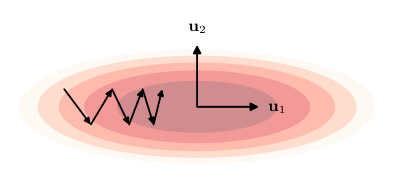
\includegraphics[width=0.4\textwidth]{figure7-3.png}
    \caption{步长固定的梯度下降}
\end{figure}

\noindent\rule{\linewidth}{0.4pt}

\section{P2}

We can gain deeper insight into the nature of this problem by considering the quadratic approximation to the error function in the neighbourhood of the minimum. From (7.7), (7.8), and (7.10), the gradient of the error function in this approximation can be written as
\begin{equation}
\nabla E = \sum_i \alpha_i \lambda_i \mathbf{u}_i.
\tag{7.24}
\end{equation}
Again using (7.10) we can express the change in the weight vector in terms of corresponding changes in the coefficients $\{\alpha_i\}$:
\begin{equation}
\Delta \mathbf{w} = \sum_i \Delta \alpha_i \mathbf{u}_i.
\tag{7.25}
\end{equation}
Combining (7.24) with (7.25) and the gradient descent formula (7.16) and using the orthonormality relation (7.9) for the eigenvectors of the Hessian, we obtain the following expression for the change in $\alpha_i$ at each step of the gradient descent algorithm:
\begin{equation}
\Delta \alpha_i = -\eta \lambda_i \alpha_i
\tag{7.26}
\end{equation}
from which it follows that
\begin{equation}
\alpha_i^{\mathrm{new}} = (1 - \eta \lambda_i) \alpha_i^{\mathrm{old}}
\tag{7.27}
\end{equation}
where `old' and `new' denote values before and after a weight update. Using the orthonormality relation (7.9) for the eigenvectors together with (7.10), we have
\begin{equation}
\mathbf{u}_i^\mathrm{T} (\mathbf{w} - \mathbf{w}^*) = \alpha_i
\tag{7.28}
\end{equation}
and so $\alpha_i$ can be interpreted as the distance to the minimum along the direction $\mathbf{u}_i$. From (7.27) we see that these distances evolve independently such that, at each step, the distance along the direction of $\mathbf{u}_i$ is multiplied by a factor $(1 - \eta \lambda_i)$. After a total of $T$ steps we have
\begin{equation}
\alpha_i^{(T)} = (1 - \eta \lambda_i)^T \alpha_i^{(0)}.
\tag{7.29}
\end{equation}
It follows that, provided $|1 - \eta \lambda_i| < 1$, the limit $T \to \infty$ leads to $\alpha_i = 0$, which from (7.28) shows that $\mathbf{w} = \mathbf{w}^*$ and so the weight vector has reached the minimum of the error.

\noindent\rule{\linewidth}{0.4pt}

\section{P3}

Note that (7.29) demonstrates that gradient descent leads to linear convergence in the neighbourhood of a minimum. Also, convergence to the stationary point requires that all the $\lambda_i$ be positive, which in turn implies that the stationary point is indeed a minimum. By making $\eta$ larger we can make the factor $(1 - \eta \lambda_i)$ smaller and hence improve the speed of convergence. There is a limit to how large $\eta$ can be made, however. We can permit $(1 - \eta \lambda_i)$ to go negative (which gives oscillating values of $\alpha_i$), but we must ensure that $|1 - \eta \lambda_i| < 1$ otherwise the $\alpha_i$ values will diverge. This limits the value of $\eta$ to $\eta < 2 / \lambda_{\max}$ where $\lambda_{\max}$ is the largest of the eigenvalues. The rate of convergence, however, is dominated by the smallest eigenvalue, so with $\eta$ set to its largest permitted value, the convergence along the direction corresponding to the smallest eigenvalue (the long axis of the ellipse in \textbf{Figure 7.3}) will be governed by
\begin{equation}
\left(1 - \frac{2 \lambda_{\min}}{\lambda_{\max}}\right)
\tag{7.30}
\end{equation}
where $\lambda_{\min}$ is the smallest eigenvalue. If the ratio $\lambda_{\min} / \lambda_{\max}$ (whose reciprocal is known as the \emph{condition number} of the Hessian) is very small, corresponding to highly elongated elliptical error contours as in \textbf{Figure 7.3}, then progress towards the minimum will be extremely slow.

\noindent\rule{\linewidth}{0.4pt}

\section{P4 7.3.1 Momentum}

One simple technique for dealing with the problem of widely differing eigenvalues is to add a \emph{momentum} term to the gradient descent formula. This effectively adds inertia to the motion through weight space and smooths out the oscillations depicted in \textbf{Figure 7.3}. The modified gradient descent formula is given by
\begin{equation}
\Delta \mathbf{w}^{(\tau-1)} = -\eta \nabla E\left(\mathbf{w}^{(\tau-1)}\right) + \mu \Delta \mathbf{w}^{(\tau-2)}
\tag{7.31}
\end{equation}
where $\mu$ is called the momentum parameter. The weight vector is then updated using (7.15).

To understand the effect of the momentum term, consider first the motion through a region of weight space for which the error surface has relatively low curvature, as indicated in \textbf{Figure 7.4}. If we make the approximation that the gradient is unchanging, then we can apply (7.31) iteratively to a long series of weight updates, and then sum the resulting arithmetic series to give
\begin{align}
\Delta \mathbf{w} &= -\eta \nabla E \{1 + \mu + \mu^2 + \ldots \} \\
&= -\frac{\eta}{1 - \mu} \nabla E
\tag{7.32}
\end{align}
\begin{equation}
\tag{7.33}
\end{equation}
and we see that the result of the momentum term is to increase the effective learning rate from $\eta$ to $\eta / (1 - \mu)$.

Figure 7.4 Caption: With a fixed learning rate parameter, gradient descent down a surface with low curvature
leads to successively smaller steps corresponding to linear convergence. In such a situation, the effect of a momentum term is like an increase in the effective learning rate parameter.

\begin{figure}[ht]\centering
    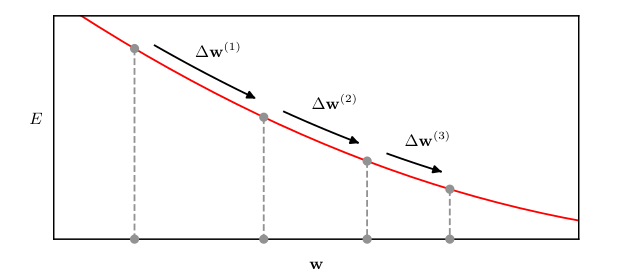
\includegraphics[width=0.4\textwidth]{figure7-4.png}
    \caption{误差曲面的曲率较低的情形}
\end{figure}

\noindent\rule{\linewidth}{0.4pt}

\section{P5}

By contrast, in a region of high curvature in which gradient descent is oscillatory, as indicated in \textbf{Figure 7.5}, successive contributions from the momentum term will tend to cancel and the effective learning rate will be close to $\eta$. Thus, the momentum term can lead to faster convergence towards the minimum without causing divergent oscillations. A schematic illustration of the effect of a momentum term is shown in \textbf{Figure 7.6}.

Figure 7.5 Caption: For a situation in which successive steps of gradient descent are oscillatory, a momentum term has little influence on the effective value of the learning rate parameter.

Figure 7.6 Caption: Illustration of the effect of adding a momentum term to the gradient descent algorithm,
showing the more rapid progress along the valley of the error function, compared with the unmodified gradient descent shown in Figure 7.3.

\begin{figure}[ht]\centering
    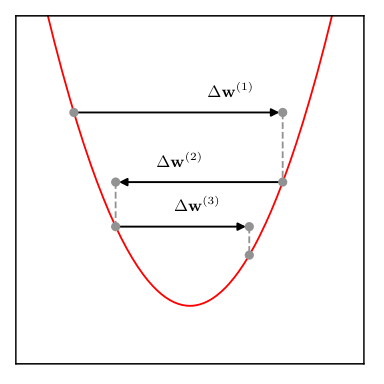
\includegraphics[width=0.4\textwidth]{figure7-5.png}
    \caption{误差曲面有较高曲率的情形}
\end{figure}

\begin{figure}[ht]\centering
    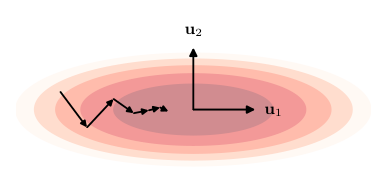
\includegraphics[width=0.4\textwidth]{figure7-6.png}
    \caption{添加动量项的梯度下降}
\end{figure}

\noindent\rule{\linewidth}{0.4pt}

\section{P6}

Although the inclusion of momentum can lead to an improvement in the performance of gradient descent, it also introduces a second parameter $\mu$ whose value needs to be chosen, in addition to that of the learning rate parameter $\eta$. From (7.33) we see that $\mu$ should be in the range $0 \leqslant \mu \leqslant 1$. A typical value used in practice is $\mu = 0.9$. Stochastic gradient descent with momentum is summarized in Algorithm 7.3.

\begin{algorithm}
\caption{7.3. Stochastic gradient descent with momentum}
\begin{algorithmic}
\Input
  \begin{minipage}[t]{0.82\linewidth}
    Training set of data points indexed by $n \in \{1,\dots,N\}$\\
    Batch size $B$\\
    Error function per mini-batch $E_{n:n+B-1}(\mathbf{w})$\\
    Learning rate parameter $\eta$\\
    Momentum parameter $\mu$\\
    Initial weight vector $\mathbf{w}$
  \end{minipage}
\Output Final weight vector $\mathbf{w}$

\noindent\rule{\linewidth}{0.05em}

\State $n \leftarrow 1$
\State $\Delta\mathbf{w} \leftarrow 0$
\Repeat
  \State $\Delta \mathbf{w} \leftarrow -\eta \nabla E_{n:n+B-1}(\mathbf{w}) + \mu\Delta \mathbf{w}$ \Comment{带动量的更新}
  \State $\mathbf{w}\leftarrow \mathbf{w} + \Delta \mathbf{w}$ \Comment{更新权重向量}
  \State $n \leftarrow n + B$
  \If{$n + B > N$}
    \State shuffle data
    \State $n \gets 1$
  \EndIf
\Until{convergence}
\State \textbf{return} $\mathbf{w}$
\end{algorithmic}
\end{algorithm}

\noindent\rule{\linewidth}{0.4pt}

\section{P7}

The convergence can be further accelerated using a modified version of momentum called \emph{Nesterov momentum} (Nesterov, 2004; Sutskever et al., 2013). In conventional stochastic gradient descent with momentum, we first compute the gradient at the current location then take a step that is amplified by adding momentum from the previous step. With the Nesterov method, we change the order of these and first compute a step based on the previous momentum, then calculate the gradient at this new location to find the update, so that
\begin{equation}
\Delta \mathbf{w}^{(\tau-1)} = -\eta \nabla E\left(\mathbf{w}^{(\tau-1)} + \mu \Delta \mathbf{w}^{(\tau-2)}\right) + \mu \Delta \mathbf{w}^{(\tau-2)}.
\tag{7.34}
\end{equation}
For batch gradient descent, Nesterov momentum can improve the rate of convergence, although for stochastic gradient descent it can be less effective.

\noindent\rule{\linewidth}{0.4pt}

\section{P8 7.3.2 Learning rate schedule}

In the stochastic gradient descent learning algorithm (7.18), we need to specify a value for the learning rate parameter $\eta$. If $\eta$ is very small then learning will proceed slowly. However, if $\eta$ is increased too much it can lead to instability. Although some oscillation can be tolerated, it should not be divergent. In practice, the best results are obtained by using a larger value for $\eta$ at the start of training and then reducing the learning rate over time, so that the value of $\eta$ becomes a function of the step index $\tau$:
\begin{equation}
\mathbf{w}^{(\tau)} = \mathbf{w}^{(\tau-1)} - \eta^{(\tau-1)} \nabla E_n(\mathbf{w}^{(\tau-1)}).
\tag{7.35}
\end{equation}

\noindent\rule{\linewidth}{0.4pt}

\section{P9}

Examples of learning rate schedules include linear, power law, and exponential decay:
\begin{align}
\eta^{(\tau)} &= \left(1 - \tau/K\right) \eta^{(0)} + (\tau/K) \eta^{(K)} \tag{7.36} \\
\eta^{(\tau)} &= \eta^{(0)} \left(1 + \tau/s\right)^c \tag{7.37} \\
\eta^{(\tau)} &= \eta^{(0)} c^{\tau/s} \tag{7.38}
\end{align}
where in (7.36) the value of $\eta$ reduces linearly over $K$ steps, after which its value is held constant at $\eta^{(K)}$. Good values for the hyperparameters $\eta^{(0)}, \eta^{(K)}, K, S,$ and $c$ must be found empirically. It can be very helpful in practice to monitor the \emph{learning curve} showing how the error function evolves during the gradient descent iteration to ensure that it is decreasing at a suitable rate.

\noindent\rule{\linewidth}{0.4pt}

\section{P10 7.3.3 RMSProp and Adam}

We saw that the optimal learning rate depends on the local curvature of the error surface, and moreover that this curvature can vary according to the direction in parameter space. This motivates several algorithms that use different learning rates for each parameter in the network. The values of these learning rates are adjusted automatically during training. Here we review some of the most widely used examples. Note, however, that this intuition really applies only if the principal curvature directions are aligned with the axes in weight space, corresponding to a locally diagonal Hessian matrix, which is unlikely to be the case in practice. Nevertheless, these types of algorithms can be effective and are widely used.

\noindent\rule{\linewidth}{0.4pt}

\section{P11}

The key idea behind \emph{AdaGrad}, short for `adaptive gradient', is to reduce each learning rate parameter over time by using the accumulated sum of squares of all the derivatives calculated for that parameter (Duchi, Hazan, and Singer, 2011). Thus, parameters associated with high curvature are reduced most rapidly. Specifically,
\begin{align}
r_i^{(\tau)} &= r_i^{(\tau-1)} + \left(\frac{\partial E(\mathbf{w})}{\partial w_i}\right)^2 \tag{7.39} \\
w_i^{(\tau)} &= w_i^{(\tau-1)} - \frac{\eta}{\sqrt{r_i^{\tau}} + \delta} \left(\frac{\partial E(\mathbf{w})}{\partial w_i}\right) \tag{7.40}
\end{align}
where $\eta$ is the learning rate parameter, and $\delta$ is a small constant, say $10^{-8}$, that ensures numerical stability in the event that $r_i$ is close to zero. The algorithm is initialized with $r_i^{(0)} = 0$. Here $E(\mathbf{w})$ is the error function for a particular mini-batch, and the update (7.40) is standard stochastic gradient descent but with a modified learning rate that is specific to each parameter.

\noindent\rule{\linewidth}{0.4pt}

\section{P12}

One problem with AdaGrad is that it accumulates the squared gradients from the very start of training, and so the associated weight updates can become very small, which can slow down training too much in the later phases. The idea behind the \emph{RMSProp} algorithm, which is short for `root mean square propagation', is to replace the sum of squared gradients of AdaGrad with an exponentially weighted average (Hinton, 2012), giving
\begin{align}
r_i^{(\tau)} &= \beta r_i^{(\tau-1)} + (1 - \beta) \left(\frac{\partial E(\mathbf{w})}{\partial w_i}\right)^2 \tag{7.41} \\
w_i^{(\tau)} &= w_i^{(\tau-1)} - \frac{\eta}{\sqrt{r_i^{\tau}} + \delta} \left(\frac{\partial E(\mathbf{w})}{\partial w_i}\right) \tag{7.42}
\end{align}
where $0 < \beta < 1$ and a typical value is $\beta = 0.9$.

\noindent\rule{\linewidth}{0.4pt}

\section{P13}

If we combine RMSProp with momentum, we obtain the \emph{Adam} optimization method (Kingma and Ba, 2014) where the name is derived from `adaptive moments'. Adam stores the momentum for each parameter separately using update equations that consist of exponentially weighted moving averages for both the gradients and the squared gradients in the form
\begin{align}
s_i^{(\tau)} &= \beta_1 s_i^{(\tau-1)} + (1 - \beta_1) \left(\frac{\partial E(\mathbf{w})}{\partial w_i}\right) \tag{7.43} \\
r_i^{(\tau)} &= \beta_2 r_i^{(\tau-1)} + (1 - \beta_2) \left(\frac{\partial E(\mathbf{w})}{\partial w_i}\right)^2 \tag{7.44} \\
\widehat{s}_i^{(\tau)} &= \frac{s_i^{(\tau)}}{1 - \beta_1^\tau} \tag{7.45} \\
\widehat{r}_i^{(\tau)} &= \frac{r_i^{(\tau)}}{1 - \beta_2^\tau} \tag{7.46} \\
w_i^{(\tau)} &= w_i^{(\tau-1)} - \eta \frac{\widehat{s}_i^{\tau}}{\sqrt{\widehat{r}_i^{\tau}} + \delta}. \tag{7.47}
\end{align}
Here the factors $1/(1 - \beta_1^\tau)$ and $1/(1 - \beta_2^\tau)$ correct for a bias introduced by initializing $s_i^{(0)}$ and $r_i^{(0)}$ to zero. Note that the bias goes to zero as $\tau$ becomes large, since $\beta_i < 1$, and so in practice this bias correction is sometimes omitted. Typical values for the weighting parameters are $\beta_1 = 0.9$ and $\beta_2 = 0.99$. Adam is the most widely adopted learning algorithm in deep learning and is summarized in Algorithm 7.4.


\begin{algorithm}
\caption{7.4. Adam optimization}
\begin{algorithmic}
\Input
  \begin{minipage}[t]{0.82\linewidth}
    Training set of data points indexed by $n \in \{1,\dots,N\}$\\
    Batch size $B$\\
    Error function per mini-batch $E_{n:n+B-1}(\mathbf{w})$\\
    Learning rate parameter $\eta$\\
    Decay parameters $\beta_1$ and $\beta_2$\\
    Stabilization parameter $\delta$
    % Initial weight vector $\mathbf{w}$
  \end{minipage}
\Output Final weight vector $\mathbf{w}$

\noindent\rule{\linewidth}{0.05em}

\State $n \leftarrow 1$
\State $s \leftarrow 0$
\State $r \leftarrow 0$
\Repeat
  \State Choose a mini-batch at random from D 
  \State $g=-\nabla E_{n:n+B-1}(w)$ \Comment{计算梯度向量}
  \State $s\leftarrow \beta_1s + (1-\beta_1)g$
  \State $r\leftarrow \beta_2r + (1-\beta_2)g\odot g$ \Comment{按分量对应相乘}
  \State $\hat{s}\leftarrow s/(1-\beta_1^\tau)$
  \State $\hat{r}\leftarrow r/(1-\beta_2^\tau)$
  \State $\Delta \mathbf{w} \leftarrow -\eta \frac{\hat{s}}{\sqrt{\hat{r}}+\delta}$
  \State $\mathbf{w}\leftarrow \mathbf{w} + \Delta \mathbf{w}$ \Comment{更新权重向量}
  \State $n \leftarrow n + B$
  \If{$n + B > N$}
    \State shuffle data
    \State $n \gets 1$
  \EndIf
\Until{convergence}
\State \textbf{return} $\mathbf{w}$
\end{algorithmic}
\end{algorithm}

\noindent\rule{\linewidth}{0.4pt}

\end{document}